% Documentclass options:
%    10pt, 11pt, 12pt  -- set type size
%    draft             -- single space, mark overfull hboxes on paper
%    final             -- double space, don't mark overfull hboxes on paper
%    oneside           -- format for one-sided printing
%    twoside           -- format for two-sided printing
% Defaults are 11pt,final,oneside.  Keep these, please.
\documentclass[11pt]{ucscthesisbs}
\bibliographystyle{apalike2}
\usepackage{natbib}
\usepackage{graphicx,epsf}% Include figure files


% The following declaration is for citations and bibliographies consistent with
% Astrophysical Journal specifications.  It may be left out or replaced with
% another bibliography/citation style.  See also the "\bibliographystyle"
% command later in this file.
%\usepackage{apj}

\usepackage{xcolor}
\usepackage{pagecolor}
\usepackage{lipsum}  

% \pagecolor{darkgray}
% \color{white}

\pagecolor{white}
\color{black}


\begin{document}

% Declarations for Front Matter

\title{Condensation-inhibited convection and thermal evolution of uranus and neptune}
\author{Robert Schroder}
\degreeyear{2020}
\degreemonth{November}
\degree{BACHELOR OF SCIENCE}
\field{ASTROPHYSICS}%
% Declare up to five committee members.  The text will be reproduced directly
% on the signature page.  Though the chair is a committee member, leave
% him/her out of the \committeemember declarations.  Make sure \numberofmembers
% agrees with the number of committee members declared INCLUDING the chair.
% If it is wrong, you will get extra or missing lines on the signature page.
%
\chair{Bruce Schumm}
\thesisadvisor{Christopher Mankovich}
\technicaladvisor{Jonathan Fortney}
\numberofmembers{3}




\campus{Santa Cruz}

\maketitle
\copyrightpage

\begin{frontmatter}

\begin{abstract}
This will be the last section written, once we have finished our analysis.
\end{abstract}

\tableofcontents
%
% The most recent (10/95) guidelines make absolutely no mention of the list
% of figures and list of tables.  Are they necessary?  If not, comment the
% next two lines out.
%
\listoffigures
\listoftables

\begin{dedication}
\null\vfil
{\large
\begin{center}
To Who,\\\vspace{12pt}
the owl
\end{center}}
\vfil\null
\end{dedication}

\begin{acknowledgements}
I'd like to thank my attorney, Bob Loblaw
\end{acknowledgements}


\end{frontmatter}

%\part{First Part}

\chapter{Introduction}
Since the work of Rupert Wildt\citep{wildt_1947}, astronomers have been modeling hydrogen dominated planets. The influential paper of the mid-twentieth century was written by Wendell DeMarcus\citep{demarcus_1958}. In this paper, DeMarcus gave a lengthy description.... Attempts at modeling the interior structure and atmosphere of the solar system giant planets significantly accelerated in the later half of the twentieth century shortly after Frank Low, confirmed by way of observation, that Jupiter was radiating more heat than it received from the Sun \citep{low_1966}. By the 1970's, modeling efforts by \citep{graboske_1975}, \citep{hubbard_1977}, and \citep{pollack_1977} for Jupiter and Saturn began incorporating model atmospheres with models of interiror structure to better investigate the thermal evolution of these giant planets. 


In section 1.1, we review prior work done on model Uranus and Neptune. In section 1.2, we review prior work done on the formation of water condensation zones in these hydrogen rich atmospheres. In chapter 2, we describe our model and present our results. In chapter 3, we discuss the ramifications of condensation inhibited convection for the thermal evolution of Uranus. Finally, in chapter 4, we summarize our findings.\citep{friedson_2017} \citep{leconte_2017} \citep{pollack_1977}\citep{fortney_2011} \citep{graboske_1975} \citep{guillot_2019} \citep{guillot_1995}

test

\section{Model Uranus and Neptune with Dry Convection}\label{model_atmosphere_background}

Will review current understanding of solar system giant planet thermal evolution here, referencing work done by Fortney, et al., and others. Not sure how far back I want to go here, but will probably mention when, and by who, thermal evolution modeling began, and then quickly get into the thermal evolution background from fortney papers.

\begin{figure}[ht!]
 \centerline{
  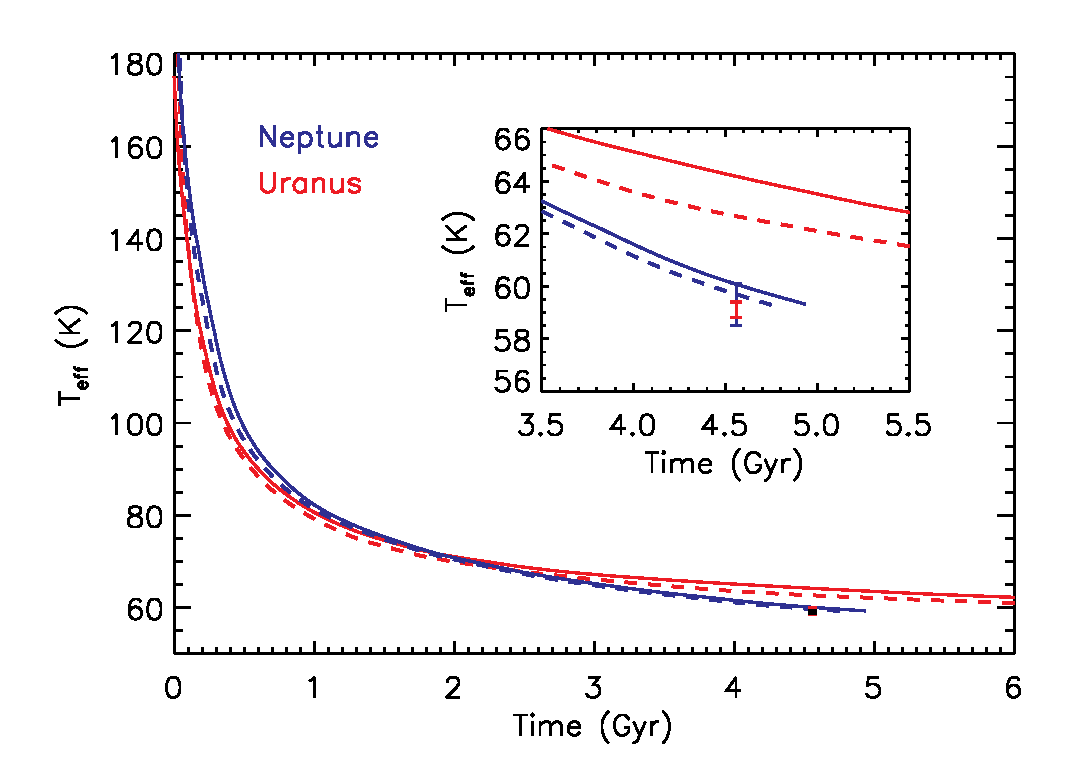
\includegraphics[width=4.0in]{figures/f10.eps}
 }
\caption[This is just a placeholder for our own plot]
{Thermal evolution of Uranus and Neptune 
}

\label{fig:discretescan}
\end{figure}


\section{Condensation-inhibited Convection}\label{condensation_background}

This section will contain theory and results surrounding condensation in hydrogen rich atmospheres, citing LeConte, Friedson, others.


\chapter{Model Uranus and Neptune with Condensation-inhibited Convection}

\section{Numerical Model}

\section{Results}

\begin{figure}[ht!]
 \centerline{
  \includegraphics[width=7.0in]{figures/convection_inhibited_2.png}
 }
\caption[Inhibition of convection on Uranus]
{Need to add description here }
\label{fig:uranus}
\end{figure}
\begin{figure}[ht!]
 \centerline{
  \includegraphics[width=7.0in]{figures/radiative_plots_1.png}
 }
\caption[Inhibition of convection on Neptune]
{Need to add description here }
\label{fig:neptune}
\end{figure}


\chapter{Discussion and Conclusions}





\appendix
\chapter{Some Ancillary Stuff}

Ancillary material should be put in appendices.  The guidelines are not
clear whether bibliography comes before or after the appendices, but they
\emph{suggest} appendices come first.
Ancillary material should be put in appendices.  The guidelines are not
clear whether bibliography comes before or after the appendices, but they
\emph{suggest} appendices come first.
Ancillary material should be put in appendices.  The guidelines are not
clear whether bibliography comes before or after the appendices, but they
\emph{suggest} appendices come first.
Ancillary material should be put in appendices.  The guidelines are not
clear whether bibliography comes before or after the appendices, but they
\emph{suggest} appendices come first.



\bibliography{wcz_bib}


\end{document}
